\cleardoublepage

\chapter{Resultados}
\label{makereference7}

Los resultados de este apartado se basan en la exploración tipo Grid descrita en el apartado anterior. Los datos utilizados en esta exploración han sido los proporcionados por InfoRiego entre el 1 de enero de 2015 hasta el 31 de diciembre del 2015.

Para llevar a cabo el entrenamiento anterior, y poder obtener una métrica con la que evaluarlo, es necesario realizar una división del conjunto de datos en dos para cada prueba. Un conjunto para entrenar el modelo y otro para comprobar la precisión de este. Es importante que estos dos conjuntos sean complementarios ya que el modelo entrenado no debe conocer ningún dato del conjunto de test o el entrenamiento se vería alterado por conocer de antemano los datos a predecir.

El tamaño de cada conjunto es también un hecho relevante ya que con un conjunto de datos muy pequeño para el entrenamiento, la predicción sería dificilmente alcanzable con éxito y con un conjunto muy grande, habría pocos datos para probar que el modelo es fiable. Una división típica es dividir el conjunto de datos en 70/30, es decir, 70\% de los datos para entrenamiento y 30\% para comprobación. En este se ha utilizado una división 25/75 que es la utilizada por defecto por el grid search de SciKitLean.

Para poder analizar los resultados, la prueba anterior proporciona distintas métricas para medir la calidad del modelo. La implementación de GridSearch utilizada (librería de scikit-learn) pretende dar una misma interfaz para utilizar esta técnica con distintos algoritmos, por lo tanto, los resultados que se obtienen con ellos también tienen una misma forma de nombrar las métricas para todos.

Sin embargo, aunque en los ficheros de resultados aparezcan los mismos nombres para medir los resultados, el significado de estos es distinto dependiendo del modelo seleccionado. En los distintos apartados dedicados a cada uno de estos modelos se explicará el significado de sus métricas.

Junto con las métricas de calidad del modelo entrenado aparecen los parámetros necesarios para obtener dicho modelo. Tanto los parámetros específicos de cada modelo como el número de instantes anteriores utilizados (``k'') o la distancia a la predicción.

A la distancia a la predicción la llamaremos ``horizonte de predicción'' y especifica la diferencia entre la hora a la que se realiza la predicción y la hora a la que se quiere predecir entre el intervalo de medida (30 minutos para estos datos). Aunque se haya probado con varios horizontes, el que más nos interesa es ``2'', que indica una predicción a una hora.

Se han realizado tres conjuntos de pruebas, una por cada algoritmo predictivo estudiado. A continuación se analizan los resultados para cada uno de estos algoritmos.

\section{Regresión Lineal}
\label{makereference7.1}
Los parámetros suministrados a GridSearch para realizar el entrenamiento con este modelo son los siguientes:

\begin{itemize}
\item Inicio: 01-01-2015
\item Fin: 31-12-2015
\item k: 2, 3, 4, 5
\item Horizonte de predicción: 2, 3, 4, 5, 6, 7
\item fit\_intercept: true, false
\item copy\_X: true, false 
\end{itemize}

Grid serach estudiará los resultados para todas las combinaciones posibles.

De los resultados obtenidos para este algoritmo mostrados en la figura \ref{resultado_linear}, la columna ``mean'' nos indican el \(R^{2}\) obtenido. \(R^{2}\) es el coeficiente de correlación y, en regresión lineal, es el cuadrado del \textit{coeficiente de correlación de Pearson}. Se calcula dividiendo el cuadrado de la covarianza del conjunto de datos reales y los predichos entre el producto de los cuadrados de la desviación típica de cada conjunto. Expresa la calidad de la predicción del modelo entre 0 y 1.

\begin{figure}[htb]
	\begin{center}
		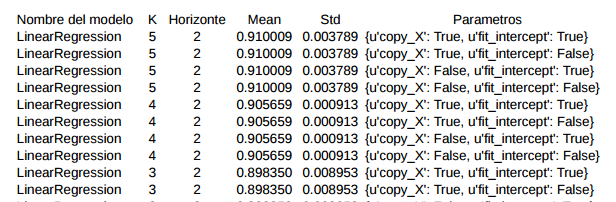
\includegraphics[width=14cm]{figures/resultado_linear.png}
		\caption{Resultado Regresión Lineal \label{resultado_linear}}
	\end{center}
\end{figure}

Los datos se muestran ordenados por la columna ``mean'' siendo así el primero de estos registros el que más coeficiente de correlación obtiene con un coeficiente de correlación de 0.910009.

Como se puede observar en la figura \ref{resultado_linear}, el modelo obtenido con mejor coeficiente de correlación tiene la siguiente configuración:

\begin{itemize}
\item Inicio: 01-01-2015
\item Fin: 31-12-2015
\item k: 5
\item Horizonte: 2
\item copy\_X: true
\item fit\_intercept: True
\end{itemize}

En el anexo \ref{Appendix:Key1} de Regresión Lineal, se muestran distintas gráficas con la radiación de este modelo durante varios días del año, la predicción que obtenemos con el modelo obtenido con mayor coeficiente de correlación y el modelo conservador.

Este ``modelo conservador'' expresa una predicción de la radiación que toma como valor, la radiación que toma como predicción la radiación en el instante anterior.

El objetivo de este proyecto es superar, como mínimo este modelo conservador.

\section{SVR}
\label{makereference7.2}

Para la exploración del modelo SVR usamos las siguientes posibles configuraciones:

Esta configuración viene reflejada en la figura \ref{json}, al igual que regresión lineal.

Para SVR se utiliza la misma métrica que la vista en el apartado anterior. Esto es porque ambas son regresiones y esta es muy utilizada en ese caso.

\section{Redes Neuronales}
\label{makereference7.3}

En la figura \ref{json_mlp} se puede observar los parámetros a explorar que usa GridSearch para determinar qué configuración del modelo de redes neuronales es mejor para nuestro proyecto:

\begin{itemize}
\item k: 2, 3, 4, 5
\item solver: ``lbfgs'', ``sgd''
\item hidden\_layer\_sizes:
	\begin{itemize}
	\item 5, 2
	\item 5, 3
	\item 5, 4
	\end{itemize}
\item random\_state: 1, 2
\end{itemize}

\begin{figure}[htb]
	\begin{center}
		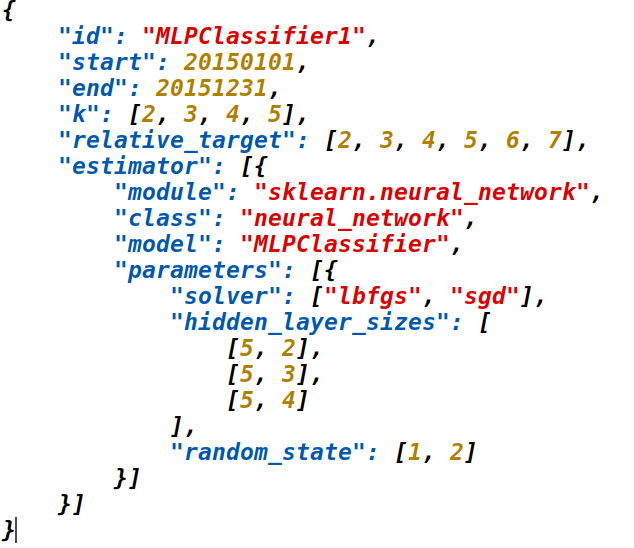
\includegraphics[width=12cm]{figures/json_mlp.png}
		\caption{Archivo de configuración para la exploración de redes neuronales \label{json_mlp}}
	\end{center}
\end{figure}

En este caso, la métrica utilizada para determinar la calidad del modelo ha sido ``accuracy'' (en español, exactitud). Es una métrica muy utilizada en clasificadores que indica el porcentaje de predicciones clasificadas correctamente.

Después de realizar la exploración de los parámetros de los distintos algoritmos de predicción explicados anteriormente (capítulo \ref{makereference5}), hemos obtenido varias métricas de cada uno de ellos.

\begin{itemize}
	\item Media
	\item Desviación estándar
\end{itemize}

Estas dos variables son las que nos dan la información necesaria para decantarnos por un modelo u otro. Buscamos aquella configuración de los parámetros que maximice la media y minimice el error.

La primera prueba que se realizó fue con algoritmos de regresión lineal y SVR.

De todos los resultados obtenidos, el que mayor media proporciona es un modelo realizado con Regresión Lineal, que obtiene una media de 0.910009 y un error de 0.003789. Su configuración es la siguiente:

\begin{itemize}
	\item k: 5
	\item distancia: 2
	\item copy\_X: ``true''
	\item fit\_intercept: ``true''
\end{itemize}

Esta media no es suficiente para afirmar que el modelo predictivo funciona. Para ello necesitaríamos una media mayor. Intuitivamente, una regresión lineal nunca sería capaz de proporcionarnos una buena predicción, ya que nuestros datos no son lineales. Ver figura \ref{modelo_verano}.

La segunda prueba se realizó con redes neuronales. Como este algoritmo es un clasificador ha sido necesario ``mapear'' las predicciones en distintas clases. Debido a que estos datos han sido normalizados, es sencillo clasificarlos en 100 clases [0, 100]. La intención de estas clases no es tanto acertar la cantidad de radiación sino proporcionar un rango en la que se encontrará.

\begin{figure}[htb]
	\begin{center}
		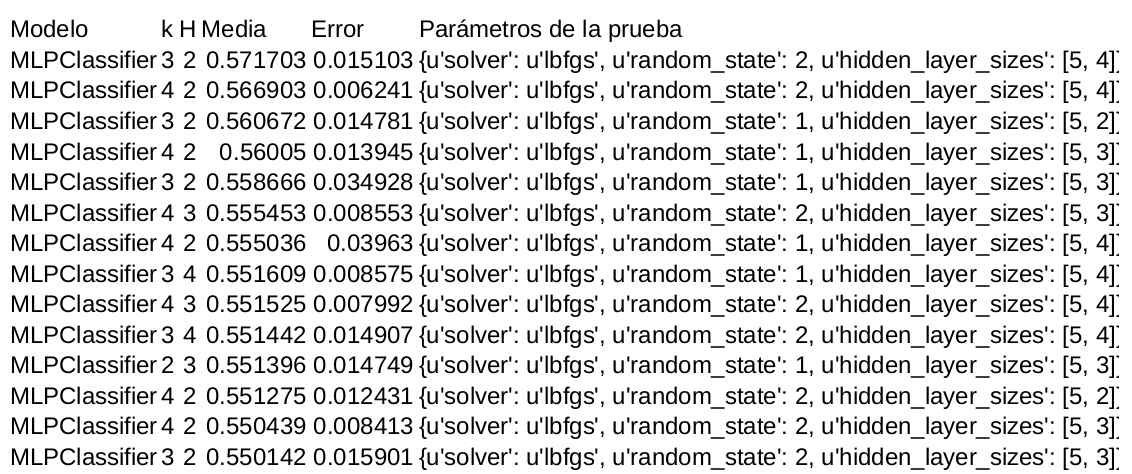
\includegraphics[width=14cm]{figures/resultado_mlp.png}
		\caption{Resultado redes neuronales \label{resultado_mlp}}
	\end{center}
\end{figure}

Una vez realizadas las pruebas, se observa que la media es muy baja,0.539901 en el mejor caso. Descartamos utilizar estos modelos de redes neuronales en nuestro proyecto.

Como futura vía de estudio se plantea volver a realizar este entrenamiento replanteando los parámetros y el ``mapeo'' de las clases.

Finalmente, hemos elegido el modelo SVR con las configuraciones siguientes:

\begin{itemize}
	\item k: 4
	\item distancia: 2
	\item kernel: ``rbf''
	\item C: 1000
	\item gamma: 0.001
\end{itemize}

\begin{figure}[htb]
	\begin{center}
		\includegraphics[width=16cm]{figures/resultado_elegido.png}
		\caption{Resultado elegido \label{resultado_elegido}}
	\end{center}
\end{figure}

Aunque no es el modelo con más media ni menos error, es de los más equilibrados. Esta configuración obtiene una media de acierto de 0.901516, distanciándose en 0.008493 de la media máxima conseguida. Su error es de 0.000330. Además se intuye que SVR debería ser el modelo que mejor se ajuste. Por lo que en un futuro estudio que busque mejorar esta predicción, sería un buen punto de partida.

\section{Calidad del código}
\label{makereference7.4}

Una vez acabado el código del proyecto, decidimos certificar su calidad mediante \href{https://www.codacy.com}{Codacy}.
Codacy es una herramienta que proporciona nuestro controlador de versiones GitHub. Sencillamente revisa todas y cada una de las líneas del código, para hacerlo más sencillo, escalable y seguro. Genera un informe con los errores y te dice qué grado de calidad tiene, siendo A el más alto. (\cite{ARP:Codacy:2017})

\begin{figure}[htb]
	\begin{center}
		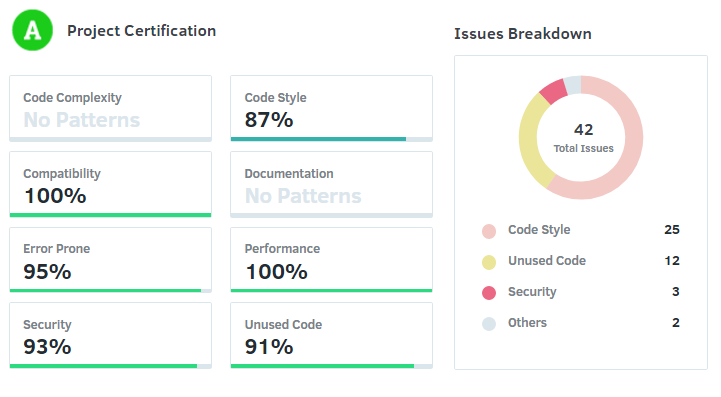
\includegraphics[height=3.5in]{figures/codacy.png}
		\caption{Informe de nuestro proyecto [Fuente: \href{https://www.codacy.com}{Codacy}] \label{codacy}}
	\end{center}
\end{figure}